% vim:set spell:
% vim:spell spelllang=fr:
\documentclass[a4paper]{article}
\usepackage[french]{babel}
\usepackage[utf8x]{inputenc}
\usepackage[T1]{fontenc}
\usepackage{libertine}
\usepackage[scaled=0.83]{beramono}
\usepackage{helvet}
\usepackage{graphicx}
\usepackage{amsmath,amssymb}
\usepackage[french]{babel}
\usepackage{xspace}
\usepackage{setspace}
\usepackage{hyperref}
\setstretch{1.0}
\usepackage{subfigure}
\voffset       -1in
\hoffset       -1in
\headheight     12pt
\headsep        12pt
\topmargin      25mm
\oddsidemargin  20mm
\textwidth      170mm
\textheight     240mm
\flushbottom
\graphicspath{{./figures/}{../../scripts/}}
\begin{document}
\begin{center}
\large
Travaux Pratiques Archi SEOC-3A - 2021/2022\\
Sujet de Frédéric Pétrot et Arthur Perais\\
\LARGE
Implantations et évaluations de\\
quelques prédicteurs de branchements\\
\large

Durée~: 4 heures
\end{center}
\section{Organisation}
Ce TP se fait soit seul, soit en binôme, à votre convenance.
Le travail demandé TP fait l'objet d'un rendu contenant un court rapport qui inclut les \emph{résultats} d'expérimentations et un \emph{tarball} (ou un git) contenant vos sources à fournir en fin de séance.
Un gabarit en \LaTeX\ qui reprend le predicteur BHT avec un compteur à saturation est donné en exemple.
Vous avez également un script fourni pour vous permettre de systématiser les simulations et l'obtention des graphes des résultats.
Ce script marche avec le prédicteur BHT qui a deux arguments, il est donc nécessaire de le modifier pour utiliser un prédicteur avec un nombre d'arguments différents.
Le sous-répetoire \verb+sle3a/rendu+ contient un exemple de .tex permettant de faire un petit rapport sur le travail.

\section{Introduction}
On cherche à étudier le comportement en situation réelle de différents prédicteurs de branchement, du plus simple au plus complexe. Pour cela, on va développer un modèle en C++ de chacun de ces prédicteurs sur lequel on fera passer un ensemble de traces d'exécutions, nous permettant d'obtenir en sortie le ratio de mauvaises prédictions (en fait le nombre de \emph{Miss Prediction per Kilo Instructions}, MPKI). On fera varier les différents paramètres du prédicteur, en particulier la taille des tables, afin d'en extraire un comportement asymptotique (par benchmark), dont on tirera un graphe.

L'infrastructure dans laquelle insérer le modèle de prédicteur est celle qui a été utilisée par le \emph{The 5th JILP Championship Branch Prediction Competition (CBP-5)}\footnote{Dont on trouvera la version originale sur \texttt{https://www.jilp.org/cbp2016/framework.html}}.
Cette infrastructure effectue la lecture des traces et l'appel à des fonctions qui implantent le prédicteur, et donne en sortie diverses statistiques dont les MPKI.

Le prédicteur par défaut dans l'archive fournie est un prédicteur bimodal à saturation «~$n$-bits~» vu en cours et rappelé en Figure~\ref{2-bit} pour le cas 2-bit. L'automate régissant chaque compteur est rappelé en Figure~\ref{bimod}.

Dans une case donnée, un branchement «~prédit pris~» aura une valeur $v\geq 2^{n-1}$ et «~prédit non pris~» aura une valeur $v<2^{n-1}$ (on note qu'il s'agit d'une convention, on pourrait très bien faire l'inverse). Nous ferons en séance une analyse rapide du code afin de comprendre comment il a été implanté dans l'infrastructure.

\begin{figure}[htb]
      \center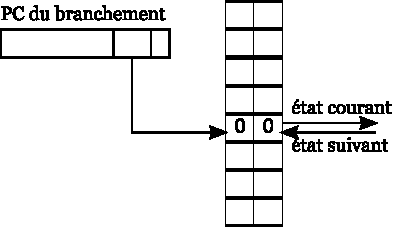
\includegraphics[scale=1]{./figures/2-bits.pdf}
      \caption{Prédicteur bimodal}
      \label{2-bit}
\end{figure}

\section{Travail demandé -- Prédicteurs simples}
On implantera différents prédicteurs en prenant soin de paramétrer les tailles afin de pouvoir lancer facilement plusieurs exécutions (\emph{cf.} l'exemple fourni) et ainsi pouvoir tracer des courbes et voir les asymptotes. \textbf{Important :} Les figures montrent souvent des prédicteurs de petites tailles, mais vous êtes invités à considérer des prédicteurs commençant au moins à 128 entrées (log2(128) = 7).

Les prédicteurs que vous devrez implanter sont les suivants~:
\begin{enumerate}
\item un prédicteur global simple, montré en Figure \ref{global-simple} avec un historique global de branchement de longueur (nombre de bits) $H$ permettant d'atteindre une entrée bimodale contenant un compteur 2-bit utilisant le graphe d'état donné en Figure \ref{bimod}. Dans le cas du prédicteur global simple, la structure contenant les prédictions est appelée \textit{Pattern History Table} (comme le premier niveau du 2-level adaptive).

      \begin{figure}[hbt]\center\leavevmode
	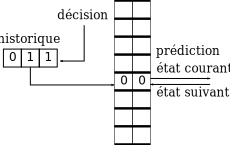
\includegraphics[scale=1]{global-simple}
	\caption{Prédicteur global simple}
	\label{global-simple}
\end{figure}


\begin{figure}[htb]
	\center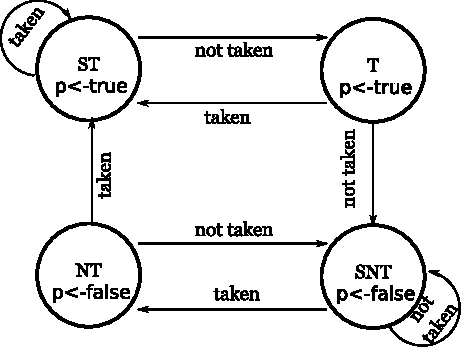
\includegraphics[scale=0.7]{./figures/2bg1.pdf}
	\caption{Automate d'un compteur 2-bit bimodal}
	\label{bimod}
\end{figure}

   L'historique global des branchements est un registre à décalage à gauche dans lequel on injecte sur le poids faible la décision prise ($H=3$ dans la figure~\ref{global-simple}).

%\item un prédicteur \emph{gshare} qui est un prédicteur global pour lequel l'index définissant l'entrée dans la table de taille $2^n$ est calculé comme le ou-exclusif d'un registre d'historique avec le pc du branchement, comme illustré sur la figure~\ref{gshare};
%      \begin{figure}[hbt]\center\leavevmode
%      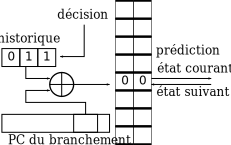
\includegraphics[scale=.9]{gshare}
%      \caption{Prédicteur \emph{gshare}}
%      \label{gshare}
%      \end{figure}
%      Si $H>n$, alors on prendra les $n$ bits de poids fort de $H$ pour faire le ou-exclusif;

\item un prédicteur \textit{gshare} qui utilise un historique global sur $H$ bits qui est combiné à l'adresse du branchement à prédire via un XOR, comme illustré sur la Figure~\ref{correlated}. On pourra tenter de trouver une fonction de hachage plus performante qu'un simple XOR;
      \begin{figure}[hbt]\center\leavevmode
      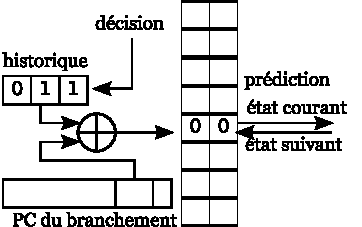
\includegraphics[scale=.9]{./figures/gshare.pdf}
      \caption{\label{correlated}Prédicteur gshare}
      \end{figure}

\item un prédicteur local qui utilise une table d'historiques sur $H$ bits (la \textit{Pattern History Table}) indexée par les poids faibles de l'adresse du branchement.  En utilisant l'entrée d'historique, on indice une BHT bimodale avec compteurs 2-bit de taille $2^H$, comme illustré sur la figure~\ref{local};
      \begin{figure}[hbt]\center\leavevmode
      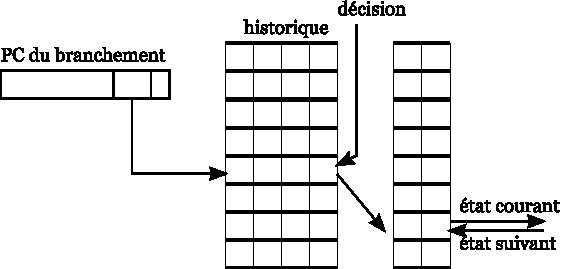
\includegraphics[scale=.9]{local}
      \caption{Prédicteur local}
      \label{local}
      \end{figure}

\item une combinaison de deux prédicteurs et le métaprédicteur associé (celui de l'alpha 21264) qui utilise un prédicteur global simple (pas gshare!) avec un historique de $H_g=12$ (soit 4096 entrées), et un prédicteur local comme celui de la précédente question, avec $H_l=10$ par entrée de la PHT (soit 1024 entrées).
La BHT indexée est un simple prédicteur bimodal, mais qui utilise des compteurs \textbf{3 bits}.

Le choix du prédicteur à utiliser se fait grâce au métaprédicteur qui comme les BHT des prédicteurs global et local contient 4K entrées de compteurs 2 bits. On accède au compteur en utilisant l'adresse du branchement à prédire, et ce compteur nous dit simplement quel prédicteur du prédicteur global ou du prédicteur local va effectuer la prédiction. Le compteur est incrémenté lorsque le prédicteur \emph{prédit} est correcte et l'autre prédicteur a fait le mauvais choix, et est décrémenté dans le cas opposé (\emph{cf.} la machine d'état de la figure~\ref{mixte-graphe}).
\begin{figure}[hbt]\center\leavevmode
      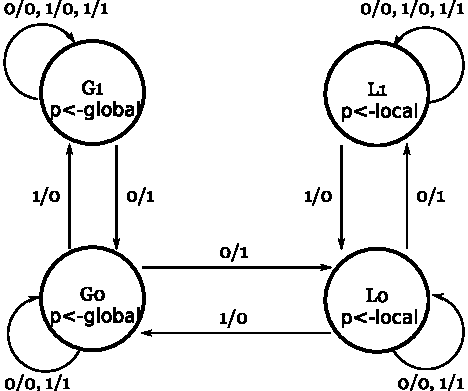
\includegraphics[scale=0.7]{./figures/mixte-graphe.pdf}
      \caption{Machine à états du choix du prédicteur.
      Légende~: $global/local$, $0$ décision incorrecte, $1$ décision correcte}
      \label{mixte-graphe}
      \end{figure}

      On ne tentera pas (du moins dans le temps imparti) de faire une version paramétrable de ce dernier prédicteur.
\end{enumerate}

Il y a un script \verb+sle3a-doit.sh+ dans le répertoire \verb+script+ qui lance automatiquement l'exécution sur un sous-ensemble des traces pour un prédicteur donné, qu'il a fallut préalablement compiler dans le répertoire \verb+sim+.
Il y a dans le script pour le prédicteur $n$-modal 2 boucles imbriquées~: la boucle externe, indice $i$, fait varier le nombre de bits du compteur, et la boucle interne, d'indice $j$, fait varier le nombre de bits de PC à utiliser pour indexer les tables.
Vous serez amené à modifier les valeurs des bornes en fonction des prédicteurs, voir à changer un peu cette partie si vous faites des prédicteurs exotiques.

Le script \verb+sle3a-doit.sh+ produit ses résultats dans \verb+../results/xxx+, ou \verb+xxx+ est un répertoire dont le nom peut-être choisi à l'envie.
Il les analyse ensuite et génère des programmes \texttt{python} qui servent à tracer des courbes (avec \texttt{matplotlib}). Ces courbes sont crées dans le répertoire où on appelle \verb+sle3a-doit.sh+ et ce sont ces courbes que l'on vous demande d'analyser. \\

On donne sur la figure~\ref{results} le type de résultat attendu pour le prédicteur n-bit.

      \begin{figure}[h]
      \centering
      \subfigure[1 bit par compteur]{
      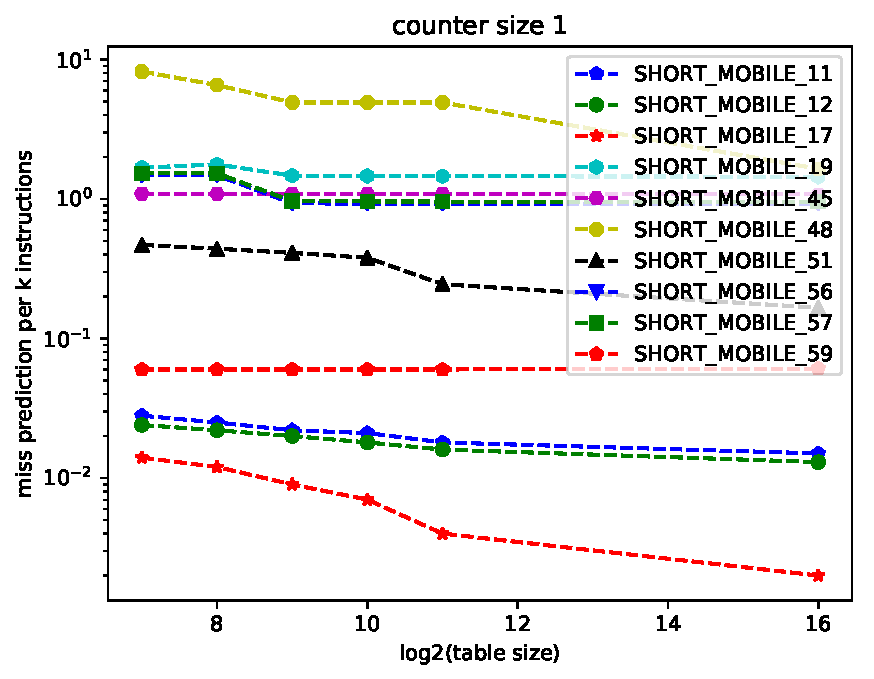
\includegraphics[scale=.48]{figures/graph_1.pdf}
      \label{plot1}
      }
      \subfigure[2 bits par compteur]{
      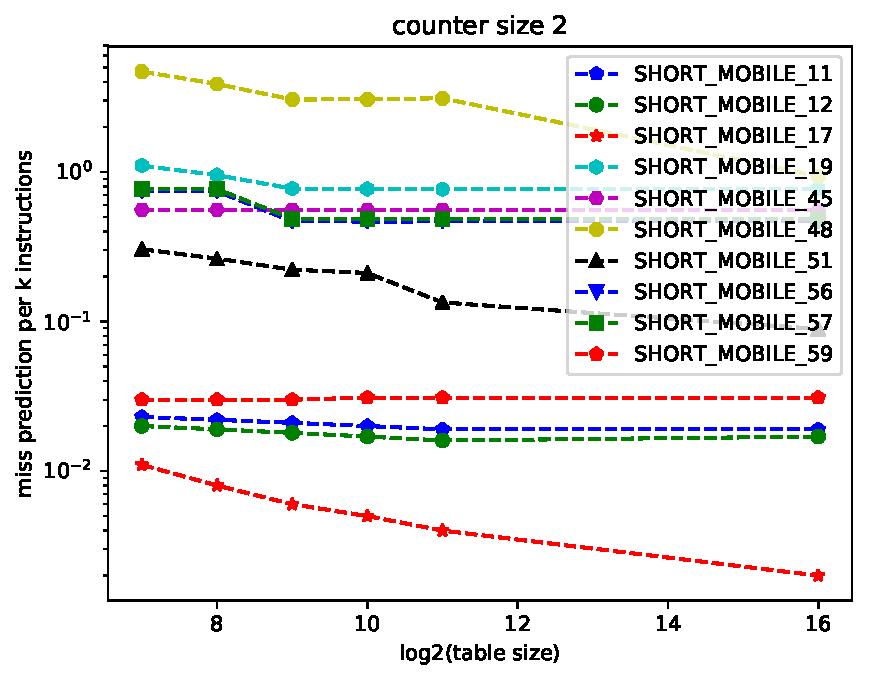
\includegraphics[scale=.48]{figures/graph_2.pdf}
      \label{plot2}
      }
      \subfigure[3 bits par compteur]{
      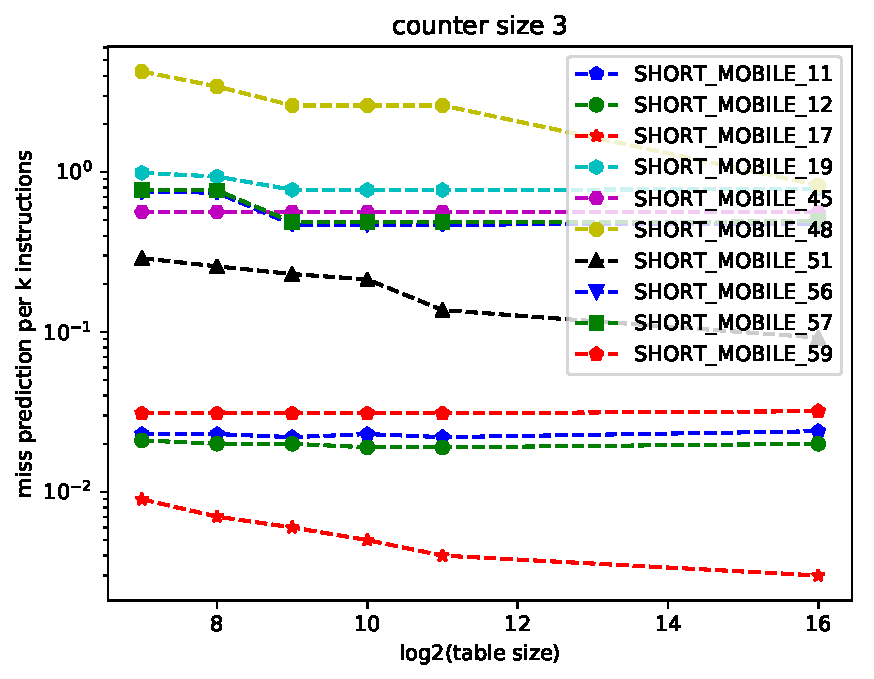
\includegraphics[scale=.48]{./figures/graph_3.pdf}
      \label{plot3}
      }
      \subfigure[4 bits par compteur]{
      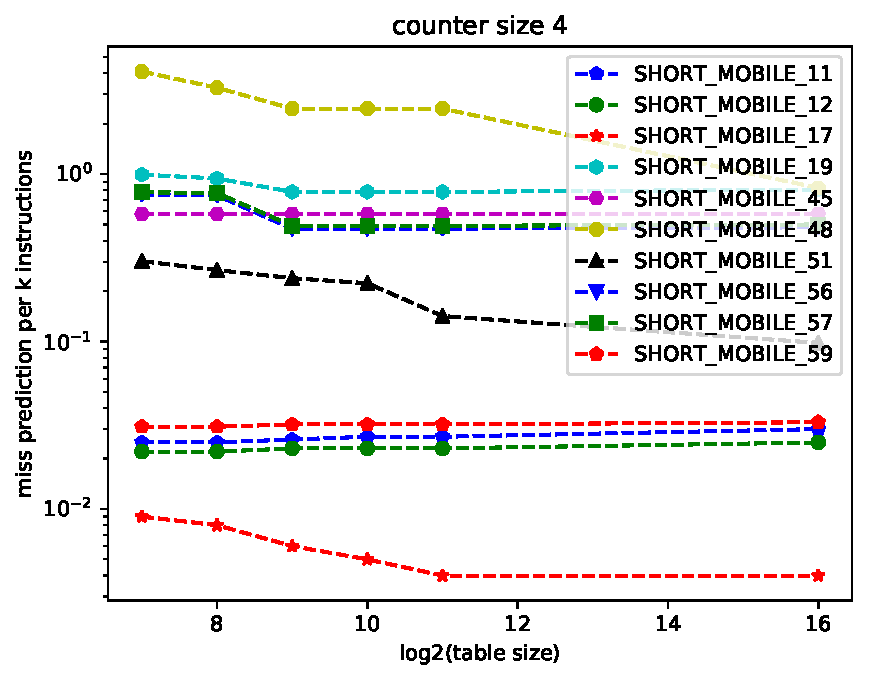
\includegraphics[scale=.48]{./figures/graph_4.pdf}
      \label{plot4}
      }
      \subfigure[5 bits par compteur]{
      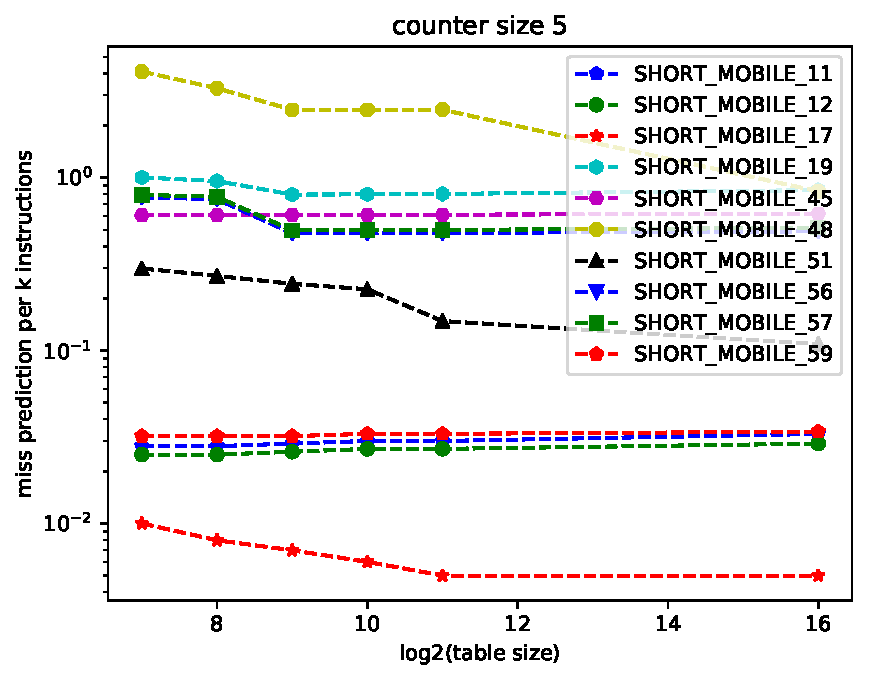
\includegraphics[scale=.48]{./figures/graph_5.pdf}
      \label{plot3}
      }
      \subfigure[6 bits par compteur]{
      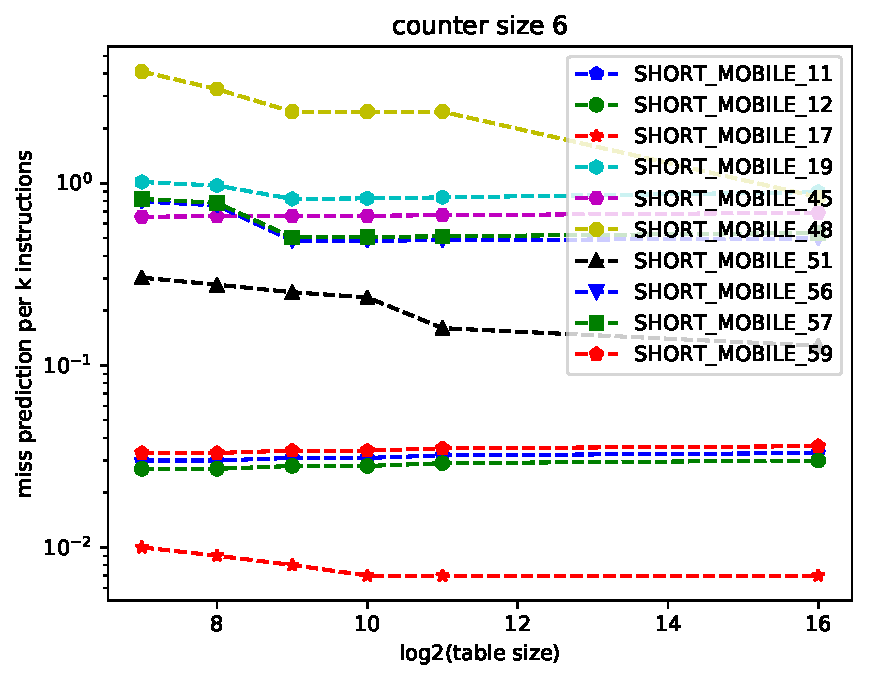
\includegraphics[scale=.48]{./figures/graph_6.pdf}
      \label{plot4}
      }
      \caption{\label{results}Les courbes de MPKI pour le prédicteur bimodal simple, en fonction du nombre de bits par compteur et du nombre d'entrées.}
      \end{figure}

\clearpage
\section{Travail demandé -- Aller plus loin}

La deuxième partie de ce TP est plus propective, car il s'agit d'améliorer la performance des prédicteurs simples implémentés jusqu'ici. On se propose de suivre deux chemins possibles. \\

\begin{enumerate}
	\item Choisir un des prédicteurs de la première partie et chercher à minimiser les MPKI par tous les moyens possibles : taille des tables, fonction de hachage, associativité, combinaisons de prédicteurs, type d'historique (dans la mesure de ce que permet le simulateur), tout est permis. Ici, on vous encourage à analyser les traces, par exemple en construisant des statistiques sur chaque branchement dans la fonction \textit{UpdatePredictor()}, afin de tenter de déterminer pourquoi un branchement est mal prédit alors qu'il a l'air régulier ou corrélé à un voisin. Dans votre rapport, il conviendra d'expliquer les techniques utilisées et vos analyses quand à ce qui fonctionne le mieux.
	\item Implémenter un prédicteur moderne tel que le prédicteur neural à base de perceptrons de Jiménez et Lin, à partir du papier de recherche éponyme (\href{https://www.cs.cmu.edu/afs/cs/academic/class/15740-f18/www/papers/hpca01-jiminez-perceptron.pdf}{Lien}, et en comparer la performance avec les prédicteurs de la première partie. A noter que pour implémenter le prédicteur, il n'est pas nécessaire de lire tout le papier de recherche. La Figure 3 ainsi que les Sections 3.2, 3.3, 3.5 et 4 sont suffisantes. Dans votre rapport, il conviendra de décrire votre implémentation afin que l'on puisse s'assurer que vous avez bien compris le papier.
\end{enumerate}

\end{document}
